\section{Funcionamento}

\subsection{Unidade Básica de Armazenamento}
\begin{figure}[H]
    \centering
    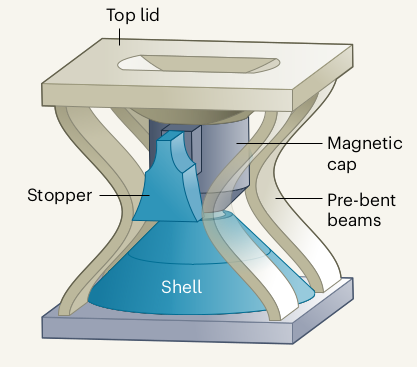
\includegraphics[scale = 0.5]{source/pictures/shell.png}
    \caption{Unidade básica de armazenamento mecânico\cite{coulais2021snappy}.}
    \label{fig:uba}
\end{figure}

A unidade básica de armazenamento mecânica possui esta estrutura, que é projeta para ter uma instabilidade de encaixe. Ela conta com dois \textit{sttopers}, que funcionam como braços para limitar a movimentação da estrutura interna e uma tampa magnética. Através dela, é possível orientar remotamente o encaixe da estrutura, por meio de um campo magnético.


\begin{figure}[H]
    \centering
    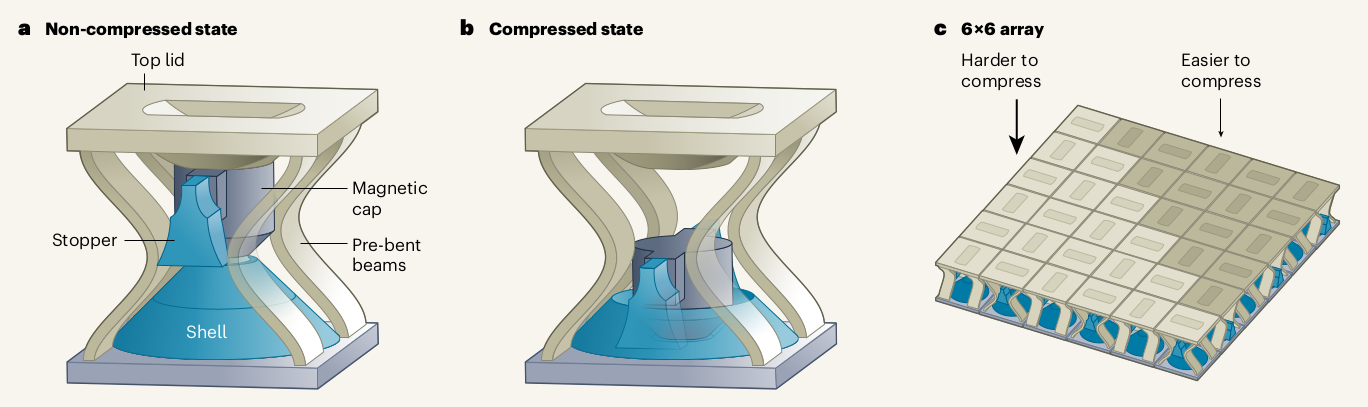
\includegraphics[width = \textwidth]{source/pictures/shell-work.png}
    \caption{Estados da UBA\cite{coulais2021snappy}.}
    \label{fig:uba-states}
\end{figure}

Nesta imagem(\ref{fig:uba-states}) é possível ver como a estrutura se altera conforme uma mudança na orientação magnética da tampa. A partir disso, é possível definir se o material é mais facilmente comprimido ou o contrário.



\subsection{Processo de gravação}

Semelhante ao disco rígido, onde o cabeçote eletromagnético orienta a polaridade da unidade básica de memória. Neste caso, um cabeçote eletromagnético vai ser responsável por orientar o estado da estrutura, como foi possível ver anteriormente.

\begin{center}
\textcolor{red}{\textbf{[VIDEO DE GRAVAÇÃO EM UBA]}}
\end{center}

Neste vídeo, é possível analisar a orientação do encaixe em uma unidade, a partir criação de um campo eletromagnético.

\begin{center}
\textcolor{red}{\textbf{[VIDEO DE GRAVAÇÃO EM ARRAY]}}
\end{center}


\section{Propriedades mecânicas dos bits}

Como foi visto anteriormente, gravar uma informação neste dispositivo gera uma alteração na estrutura das unidades que o compõem. No video a seguir é possível ver o comportamento de uma unidade diante de uma compressão em seus dois estados. 

\begin{center}
\textcolor{red}{\textbf{[VIDEO DE TESTE DE COMPRESSIBILIDADE DE UMA UNIDADE DE GRAVAÇÃO]}}
\end{center}
    
Agora em um material formado por estas unidades. 

\begin{center}
\textcolor{red}{\textbf{[VIDEO DE TESTE DE COMPRESSIBILIDADE EM UM MATERIAL FORMADOS POR ESTAS UNIDADES]}}
\end{center}

Desse modo, é possível ver como podemos controlar o comportamento de um material por meio da gravação de informações nele. 